\chapter{AFABL: A Friendly Adaptive Behavior Language}\label{ch:afabl}

\section{Background}

\subsection{Why a Domain-Specific Embedded Language?}

\subsection{Why Scala?}

\section{AFABL Concepts}

\subsection{Terminology}

\begin{itemize}

\item State

  A state is a configuration of all objects and agents in a world.
  These configurations can include object locations and orientations,
  mental or emotional dispositions of agents, or indications of the
  occurrence of events (e.g., agent X just got shot).

\item Perception, or Percept

  A subset of a world state that is perceived by an agent.

\item Action

  An action is a one-shot state manipulation that can be executed by
  an agent.  Sometimes called "primitives," actions acquire greater
  meaning when they are executed (possibly in sequences) by behavior
  modules to achieve a goal or satisfy a constraint.

\item Task

  A task is a temporally-extended action, a "mini-policy" that acheives a
  subgoal.  Tasks are equivalent to subtasks (MaxQ), abstract machines
  (PHAM), or options from hierarchical reinforcement learning.

\item World

  Sometimes called an "environment," a world is a container for all
  the things an agent can perceive and act upon, and possibly hidden
  things.  Worlds are represented by states that specify the
  configuration of all the things in a world at a given point in time.

\item World Dynamics

  The dynamics of a world specifies the state transitions that are
  made in response to the execution of actions.  World dynamics may be
  deterministic or stochastic.  Markov Decision Processes are often
  used to represent world dynamics.

\item Behavior Module

  A behavior module is a self-contained agent component that
  recommends an action (response) for a given state perception
  (stimulus).  Anything that produces a policy (a mapping from states
  to actions and tasks) is a behavior module.  A behavior module is
  sometimes called a "subagent" in modular reinforcement learning.

\item Constraint Module

  A constraint module is a behavior module that runs throughout the
  life of its containing agent and represents a state that an agent
  should constantly avoid.  It is a constraint in the sense that, in
  certain states, a constraint module will identify actions that should
  *not* be executed.

\item Drive Module

  A drive module is a behavior module that runs throughout the
  life of its containing agent and represents states that an agent
  should constantly seek.

\item Objective

  A an objective is a short-term goal state that generates a drive
  module that is active until its goal is achieved.  The command
  arbitrator gives objective modules priority over drive modules, but
  all modules are constrained by constraint modules.

\item Agent

  An agent is an entity that acts under its own control, perceiving
  the state of its world and executing actions in response to these
  perceived states.

\item Intelligent Agent

  An intelligent agent is an agent that chooses its actions to achieve
  goals or satisfy constraints.

\item Adaptive Agent

  An adaptive agent is an intelligent agent that can automatically
  adapt its behaviors to different worlds (that is, choose different
  actions sequences to achieve goals in worlds with different
  dynamics), or adapt its behaviors at run-time to worlds in which the
  dynamics change.

\item Modular Agent

  A modular agent is an agent that consists of multiple behavior
  modules and performs command arbitration to decide which module's
  preferred action to execute in a given state.

\item Command Arbitration

  Command arbitration is the act of deciding, for a given state, which
  behavior module's preferred action to execute in a given state.
\end{itemize}

\subsection{Agent Architecture}

An AFABL agent is a behavorial agent that is composed of reusable
behavior modules.  By "behavioral agent" we mean that the agent
executes an action in resopnse to a stimulus, represented by a state
observation.  Each behavior module is itself an agent that has a
preferred action for each state.  AFABL agents perform command
arbitration to choose one of the modules' recommended actions for each
state.  The behavior modules recommend actions in each state, and the
arbitrator chooses which module to "listen to" in each state.  The
AFABL agent architecture is a subsumption architecture.

\subsubsection{Behavior Modules}

Behavior modules, sometimes called subagents in the modular
reinforcement learning iterature, are agents that are meant to be
combined to form larger agents.  Behavior modules are similar to the
layers of Brooks's subsumption architecture with an important
difference: autonomy.  The internal working of a behavior module is
never altered externally.  A behavior module defines a state
abstraction that converts the state observation it is given to a
(possibly) simpler state that is used internally for decision making
and learning.  The decision making and adaptation mechanisms inside a
module remain completely under the module's control.  Interaction with
the module consists entirely of reporting a state observation to the
module, asking the module for an action, and reporting to the module
the effect of executing an action.



\subsubsection{Adaptive Modules}

An adaptive module employs learning algorithms under the hood to
achieve automatic adaptivity.  By adaptive we mean two things: (1)
adaptation to new worlds, and (2) run-time adaptaion.  A module that
is programmed to work for worlds with a given state representation
will work with any world that provides the same (or greater) state
representation, even if the dynamics of the worlds differ.  An
adaptive module need simply be retrained for the new world.  Once an
adaptive module is running in an active agent, the module may continue
to tune its internal learning models as the agent acts in the world,
providing for run-time adaptation.

\subsubsection{Command Arbitrators}

Command arbitrators take as input the action preferences of a set of
modules, and selects one of the actions.  If the command arbitrator is
part of a module, the action selected is the preferred actoin of the
module.  If the command arbitrator is part of the top-level agent,
then the actoin selected is the action that will be executed by the
agent.

\paragraph{Knowledge-Based Arbitrators}

A knowledge-based arbitrator uses hand-coded logic to decide from
among the actions recommended by a set of modules.  Simple arbetrators
with few modules to arbitrate can often be coded quite simply as
knowledge-based arbitrators.  For example, consider an arbitrator for
a simple agent consisting of two modules: AvoidWolf and FindFood.  A
command arbitrator could contain simple logic to encode the rule "when
the wolf is near, choose AvoidWolf's action, otherwise choose
FindFood's action."


\paragraph{Adaptive Arbitrators}

Adaptive arbitrators use learning algorithms under the hood to
automatically select actions from among a set of candidate actions.
Like adaptive behavior modules, adpative arbitrators must be trained
in the world with the set of modules it must arbitrate.  In effect, an
adaptvei arbitrator learns which module to listen to in a given state.


\subsubsection{Integrated Intelligence}

Because an AFABL agent performs command arbitration over modules that
support a behavioral interface (providing an action given a state
observation), the modules themselves can employ any mechanism to
decide on actions given a state.  This information hiding means that
AFABL agents can be composed of a mixture of modules that use many
different kinds of AI, including statistical learning, rule-based
reasoning, or (reactive) planning.  AFABL is an integrated
intelligence architecture.



\subsubsection{Hierarchical Decomposition}


Beacuse modules are themselves agents, modules can contain other
modules and perform command arbitration over those modules just as the
top-level agent does.  Agents can thus be decomposed recursively into
behavioral subsystems.  This recursive behavior module decomposition
provides the agent designer with great flexibility.  Recursive module
composition is somewhat similar to the levels of competence in
Brooks's subsumption architecture with an important difference: the
internal workings of modules are never altered externally.  Modules
are treated as black-boxes.  Command arbitration accomplishes the same
result that output suppression does in classic subsumption.

\section{Reinforcement Learning in AFABL}

\subsection{AFABL Agents and Reinforcement Learning Agents}

\subsection{Modular Reinforcement Learning}

\subsection{Hierarchical Reinforcement Learning}

\subsection{Automatic Adaptation}

\section{An Illustrative AFABL Agent}


\section{Adaptive Agent Software Engineering with AFABL}


\section{Software Reuse with AFABL}

AFABL supports agent-based software abstractions that permit code to be reused in new domains.  This reuse is what we mean by adaptivity: existing AFABL code can adapt to new domains without modifying the code.  We will quantify the value of this reuse in a series of
experiments described below.

\section{Experiments}

Programmers will be randomly assigned to two equally-sized groups: one group will use Scala without AFABL first -- the Scala-first group -- and the other group will use Scala with AFABL first -- the AFABL-first group.  Each group will complete three programming tasks using Scala and AFABL in the order determined by their group.  For each task the programmers will be asked to design and implement elegant code that meets the requirements of the task as quickly as possible, balancing the quality of their solutions with time.  The idea is to get a good solution quickly, not a perfect solution in a long time.

\subsection{Task 1: The Bunny-Wolf Domain}\label{sec:task1}

\begin{figure}[h]

\begin{center}
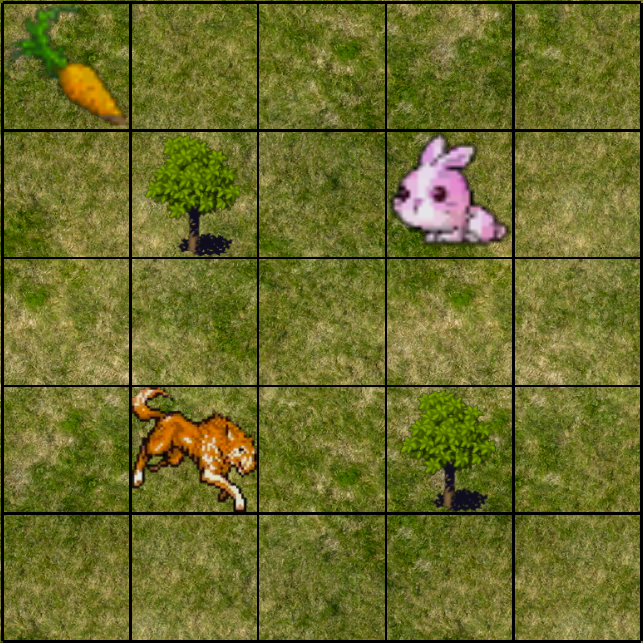
\includegraphics[height=2.4in]{bunny.png}
\end{center}


\caption{In the grid world above, the bunny must pursue two goals
  simultaneously: find food and avoid the wolf.  The bunny may move
  north, south, east, or west.  When it finds food it consumes the
  food and new food appears elsewhere in the grid world, when it meets
  the wolf it is eaten and ``dies.''}
\label{fig:bunny-picture}
\end{figure}

In this task each programmer will write an agent that controls a bunny character in a simple
world, depicted in Figure~\ref{fig:bunny-picture}.  The bunny world works as follows:

\begin{itemize}

\item The bunny world is a discrete grid of cells.  The bunny, wolf, and food each occupy one cell.

\item During each time step the bunny may move north, south, east, or west.

\item Every two time steps the wolf moves towards the bunny.

\item If the bunny moves to the cell currently occupied by the food, the bunny eats the food, receives a signal from the simulation that it has eaten the food, and new food appears elsewhere.

\item If the wolf moves to the cell currently occupied by the bunny it eats the bunny and the episode ends.

\end{itemize}

The simulation runs several episodes, keeping track of how much food the bunny eats and how long (how many time steps) the bunny ``lives'' in each episode.  Programmers will be asked to write bunny agents that live as long as possible and eat as much food as possible.

\subsection{Task 2: Mating Bunny}\label{sec:task2}

In this task each programmer will write a bunny agent for a world that is identical to the world in Task 1 except that the bunny must also find mates.  The world will include one static  potential mate that behaves similarly to the food.  When the bunny finds the potential mate, the bunny receives a signal that it has ``mated,'' the mate disappears (because it goes off to have babies), and another potential mate appears elsewhere.  The simulation runs as in Task 1, additionally keeping track of how many mates the bunny finds.  As in Task 1, programmers will be asked to write bunny agents that live as long as possible, eat as much food as possible, and find as many mates as possible.

\subsection{Task 3: Adding Wind, Spoiling Food, and Picky Mates}\label{sec:task3}

In this task each programmer will write a bunny agent for a world with the same elements as in Task 2 and with the same goals for the bunny, but the world is more complex.  In particular:

\begin{itemize}

\item There is constant wind from an unchanging direction that affects the wolf's ability to find the bunny.  The wolf will only move toward the bunny if the wolf is downwind of the bunny.

\item If food is not eaten within 15 time steps after it appears, it spoils.  Spoilage is represented by the food disappearing and new food appearing elsewhere.

\item To simulate selection of fit bunnies, potential mates will only accept the bunny if the bunny has eaten within 10 time steps (a hungry bunny is an unsuccessful bunny and therefore not fit for mating).  Rejection will be represented by the potential mate remaining in place and the bunny not receiving a signal that mating has occurred.

\end{itemize}


\subsubsection{Source Code Analysis}

The code submitted for each task will be analyzed to determine:

\begin{itemize}
\item How much code was required for each task with and without AFABL.
\item How consistent the solutions were between programmers in each task with and without AFABL.  Did AFABL lead to more consistent designs?
\item How well the programmers understood the problem.
\end{itemize}

\section{Evaluation}

The primary quantitative metric will be task completion effort in time and code quantity.  Tasks 2 and 3 will provide a measure of how much effort is required to adapt agents to new domains.  In addition, we will calculate qualitative metrics for programmer satisfaction, and mine the source code for design patterns.


\section{Conclusions}

{\bf Finding the NPC Authorability Sweet Spot with AFABL}

AFABL's integrated reinforcement learning separates the dynamics of the world from the action-slection logic in the agent, freeing the programmer from writing domain-dependent code and facilitating the adaptiation of agents to new worlds.

\begin{itemize}
\item Domain knowledge: as much or as little as you want.  You can program the parts you know how to program, and leave AFABL to learn the rest automatically.
\item Algorithm knowledge: moderate.  AFABL is based on the agent and
  reinforcement learning models.  Behaviors are programmed as actions
  that execute in response to observed state (hence ``behavior''), and
  automatic behaviors additionally specify reward signals that enable
  AFABL to learn the best responses to particular states.
\item Adaptability: high.
\end{itemize}


\subsection{Contributions}

\begin{itemize}
\item AFABL, an adaptive agent programming framework/DSL that integrates MRL into the Scala language.
\item Idioms and design patterns for using AFABL to program adaptive agents.
\item Exploratory knowledge on the kinds of framework/language features and debugging tools that are useful in adaptive partial-programming, the roles they play in the development process, and the benefits they provide.
\item Confirmatory knowledge that a programming language integrating MRL provides measurable adaptivity benefits for appropriate agent programming problems.
\end{itemize}
